% Options for packages loaded elsewhere
% Options for packages loaded elsewhere
\PassOptionsToPackage{unicode}{hyperref}
\PassOptionsToPackage{hyphens}{url}
\PassOptionsToPackage{dvipsnames,svgnames,x11names}{xcolor}
%
\documentclass[
  letterpaper,
  DIV=11,
  numbers=noendperiod]{scrartcl}
\usepackage{xcolor}
\usepackage{amsmath,amssymb}
\setcounter{secnumdepth}{-\maxdimen} % remove section numbering
\usepackage{iftex}
\ifPDFTeX
  \usepackage[T1]{fontenc}
  \usepackage[utf8]{inputenc}
  \usepackage{textcomp} % provide euro and other symbols
\else % if luatex or xetex
  \usepackage{unicode-math} % this also loads fontspec
  \defaultfontfeatures{Scale=MatchLowercase}
  \defaultfontfeatures[\rmfamily]{Ligatures=TeX,Scale=1}
\fi
\usepackage{lmodern}
\ifPDFTeX\else
  % xetex/luatex font selection
\fi
% Use upquote if available, for straight quotes in verbatim environments
\IfFileExists{upquote.sty}{\usepackage{upquote}}{}
\IfFileExists{microtype.sty}{% use microtype if available
  \usepackage[]{microtype}
  \UseMicrotypeSet[protrusion]{basicmath} % disable protrusion for tt fonts
}{}
\makeatletter
\@ifundefined{KOMAClassName}{% if non-KOMA class
  \IfFileExists{parskip.sty}{%
    \usepackage{parskip}
  }{% else
    \setlength{\parindent}{0pt}
    \setlength{\parskip}{6pt plus 2pt minus 1pt}}
}{% if KOMA class
  \KOMAoptions{parskip=half}}
\makeatother
% Make \paragraph and \subparagraph free-standing
\makeatletter
\ifx\paragraph\undefined\else
  \let\oldparagraph\paragraph
  \renewcommand{\paragraph}{
    \@ifstar
      \xxxParagraphStar
      \xxxParagraphNoStar
  }
  \newcommand{\xxxParagraphStar}[1]{\oldparagraph*{#1}\mbox{}}
  \newcommand{\xxxParagraphNoStar}[1]{\oldparagraph{#1}\mbox{}}
\fi
\ifx\subparagraph\undefined\else
  \let\oldsubparagraph\subparagraph
  \renewcommand{\subparagraph}{
    \@ifstar
      \xxxSubParagraphStar
      \xxxSubParagraphNoStar
  }
  \newcommand{\xxxSubParagraphStar}[1]{\oldsubparagraph*{#1}\mbox{}}
  \newcommand{\xxxSubParagraphNoStar}[1]{\oldsubparagraph{#1}\mbox{}}
\fi
\makeatother

\usepackage{color}
\usepackage{fancyvrb}
\newcommand{\VerbBar}{|}
\newcommand{\VERB}{\Verb[commandchars=\\\{\}]}
\DefineVerbatimEnvironment{Highlighting}{Verbatim}{commandchars=\\\{\}}
% Add ',fontsize=\small' for more characters per line
\usepackage{framed}
\definecolor{shadecolor}{RGB}{241,243,245}
\newenvironment{Shaded}{\begin{snugshade}}{\end{snugshade}}
\newcommand{\AlertTok}[1]{\textcolor[rgb]{0.68,0.00,0.00}{#1}}
\newcommand{\AnnotationTok}[1]{\textcolor[rgb]{0.37,0.37,0.37}{#1}}
\newcommand{\AttributeTok}[1]{\textcolor[rgb]{0.40,0.45,0.13}{#1}}
\newcommand{\BaseNTok}[1]{\textcolor[rgb]{0.68,0.00,0.00}{#1}}
\newcommand{\BuiltInTok}[1]{\textcolor[rgb]{0.00,0.23,0.31}{#1}}
\newcommand{\CharTok}[1]{\textcolor[rgb]{0.13,0.47,0.30}{#1}}
\newcommand{\CommentTok}[1]{\textcolor[rgb]{0.37,0.37,0.37}{#1}}
\newcommand{\CommentVarTok}[1]{\textcolor[rgb]{0.37,0.37,0.37}{\textit{#1}}}
\newcommand{\ConstantTok}[1]{\textcolor[rgb]{0.56,0.35,0.01}{#1}}
\newcommand{\ControlFlowTok}[1]{\textcolor[rgb]{0.00,0.23,0.31}{\textbf{#1}}}
\newcommand{\DataTypeTok}[1]{\textcolor[rgb]{0.68,0.00,0.00}{#1}}
\newcommand{\DecValTok}[1]{\textcolor[rgb]{0.68,0.00,0.00}{#1}}
\newcommand{\DocumentationTok}[1]{\textcolor[rgb]{0.37,0.37,0.37}{\textit{#1}}}
\newcommand{\ErrorTok}[1]{\textcolor[rgb]{0.68,0.00,0.00}{#1}}
\newcommand{\ExtensionTok}[1]{\textcolor[rgb]{0.00,0.23,0.31}{#1}}
\newcommand{\FloatTok}[1]{\textcolor[rgb]{0.68,0.00,0.00}{#1}}
\newcommand{\FunctionTok}[1]{\textcolor[rgb]{0.28,0.35,0.67}{#1}}
\newcommand{\ImportTok}[1]{\textcolor[rgb]{0.00,0.46,0.62}{#1}}
\newcommand{\InformationTok}[1]{\textcolor[rgb]{0.37,0.37,0.37}{#1}}
\newcommand{\KeywordTok}[1]{\textcolor[rgb]{0.00,0.23,0.31}{\textbf{#1}}}
\newcommand{\NormalTok}[1]{\textcolor[rgb]{0.00,0.23,0.31}{#1}}
\newcommand{\OperatorTok}[1]{\textcolor[rgb]{0.37,0.37,0.37}{#1}}
\newcommand{\OtherTok}[1]{\textcolor[rgb]{0.00,0.23,0.31}{#1}}
\newcommand{\PreprocessorTok}[1]{\textcolor[rgb]{0.68,0.00,0.00}{#1}}
\newcommand{\RegionMarkerTok}[1]{\textcolor[rgb]{0.00,0.23,0.31}{#1}}
\newcommand{\SpecialCharTok}[1]{\textcolor[rgb]{0.37,0.37,0.37}{#1}}
\newcommand{\SpecialStringTok}[1]{\textcolor[rgb]{0.13,0.47,0.30}{#1}}
\newcommand{\StringTok}[1]{\textcolor[rgb]{0.13,0.47,0.30}{#1}}
\newcommand{\VariableTok}[1]{\textcolor[rgb]{0.07,0.07,0.07}{#1}}
\newcommand{\VerbatimStringTok}[1]{\textcolor[rgb]{0.13,0.47,0.30}{#1}}
\newcommand{\WarningTok}[1]{\textcolor[rgb]{0.37,0.37,0.37}{\textit{#1}}}

\usepackage{longtable,booktabs,array}
\usepackage{calc} % for calculating minipage widths
% Correct order of tables after \paragraph or \subparagraph
\usepackage{etoolbox}
\makeatletter
\patchcmd\longtable{\par}{\if@noskipsec\mbox{}\fi\par}{}{}
\makeatother
% Allow footnotes in longtable head/foot
\IfFileExists{footnotehyper.sty}{\usepackage{footnotehyper}}{\usepackage{footnote}}
\makesavenoteenv{longtable}
\usepackage{graphicx}
\makeatletter
\newsavebox\pandoc@box
\newcommand*\pandocbounded[1]{% scales image to fit in text height/width
  \sbox\pandoc@box{#1}%
  \Gscale@div\@tempa{\textheight}{\dimexpr\ht\pandoc@box+\dp\pandoc@box\relax}%
  \Gscale@div\@tempb{\linewidth}{\wd\pandoc@box}%
  \ifdim\@tempb\p@<\@tempa\p@\let\@tempa\@tempb\fi% select the smaller of both
  \ifdim\@tempa\p@<\p@\scalebox{\@tempa}{\usebox\pandoc@box}%
  \else\usebox{\pandoc@box}%
  \fi%
}
% Set default figure placement to htbp
\def\fps@figure{htbp}
\makeatother





\setlength{\emergencystretch}{3em} % prevent overfull lines

\providecommand{\tightlist}{%
  \setlength{\itemsep}{0pt}\setlength{\parskip}{0pt}}



 


\KOMAoption{captions}{tableheading}
\makeatletter
\@ifpackageloaded{caption}{}{\usepackage{caption}}
\AtBeginDocument{%
\ifdefined\contentsname
  \renewcommand*\contentsname{Table of contents}
\else
  \newcommand\contentsname{Table of contents}
\fi
\ifdefined\listfigurename
  \renewcommand*\listfigurename{List of Figures}
\else
  \newcommand\listfigurename{List of Figures}
\fi
\ifdefined\listtablename
  \renewcommand*\listtablename{List of Tables}
\else
  \newcommand\listtablename{List of Tables}
\fi
\ifdefined\figurename
  \renewcommand*\figurename{Figure}
\else
  \newcommand\figurename{Figure}
\fi
\ifdefined\tablename
  \renewcommand*\tablename{Table}
\else
  \newcommand\tablename{Table}
\fi
}
\@ifpackageloaded{float}{}{\usepackage{float}}
\floatstyle{ruled}
\@ifundefined{c@chapter}{\newfloat{codelisting}{h}{lop}}{\newfloat{codelisting}{h}{lop}[chapter]}
\floatname{codelisting}{Listing}
\newcommand*\listoflistings{\listof{codelisting}{List of Listings}}
\makeatother
\makeatletter
\makeatother
\makeatletter
\@ifpackageloaded{caption}{}{\usepackage{caption}}
\@ifpackageloaded{subcaption}{}{\usepackage{subcaption}}
\makeatother
\usepackage{bookmark}
\IfFileExists{xurl.sty}{\usepackage{xurl}}{} % add URL line breaks if available
\urlstyle{same}
\hypersetup{
  pdftitle={DWI RD Project},
  colorlinks=true,
  linkcolor={blue},
  filecolor={Maroon},
  citecolor={Blue},
  urlcolor={Blue},
  pdfcreator={LaTeX via pandoc}}


\title{DWI RD Project}
\author{}
\date{}
\begin{document}
\maketitle


\begin{enumerate}
\def\labelenumi{\arabic{enumi}.}
\item
  \textbf{Introduction}

  Drunk driving continues to impose substantial social and economic
  costs, and legal sanctions are intended to deter repeat offenses. Yet
  it is difficult to determine whether harsher punishment actually
  reduces recidivism because drivers who receive more severe penalties
  often differ systematically from those who receive lighter ones. This
  paper examines whether crossing the legal blood alcohol concentration
  (BAC) threshold of 0.08, which triggers stricter DUI penalties,
  affects the probability that a driver commits another drunk-driving
  offense. We exploit the fact that the 0.08 rule creates a sharp policy
  cutoff: drivers just below and just above the threshold should be
  similar in underlying characteristics, but those above the cutoff face
  harsher legal consequences. Using a regression discontinuity design,
  we compare drivers near this threshold to estimate the local causal
  effect of the policy. By focusing on observations close to the cutoff,
  the analysis treats the legal threshold as a natural experiment that
  helps isolate the deterrent impact of stricter DUI punishment on
  future recidivism.
\item
  \textbf{Background and policy context.}

  In Washington State, the legal DUI threshold for adults has been BAC
  0.08 since January 1, 1999. Drivers at or above that cutoff face a DUI
  charge and substantially harsher statutory sanctions than drivers just
  below it, including higher minimum fines, mandatory jail time or home
  monitoring, license suspension, and insurance requirements. For a
  first offense, the statutory minimum penalty rises from \$865.50 with
  24 hours minimum jail and a 90-day license suspension at BAC
  0.08--0.15, with sanctions structured to escalate further for repeat
  offenders. Because punishment changes discretely at 0.08 while drivers
  very near the cutoff should otherwise be similar, crossing that
  threshold creates the policy discontinuity that makes the regression
  discontinuity design plausible in this setting.
\item
  \textbf{Data}

  We use the DWI\_Data.rdata subset of Hansen's Washington State
  impaired-driving data, which contains 214,558 traffic stops in our
  working sample and is designed to study whether harsher punishment
  affects later recidivism. The key variables are the two BAC measures,
  \texttt{bac1} and \texttt{bac2}, the outcome \texttt{recidivism}, and
  predetermined covariates including \texttt{male}, \texttt{white},
  \texttt{aged}, \texttt{acc}, and \texttt{year}. Each driver receives
  two BAC tests, so to construct a single running variable for the RD
  design we use \texttt{bac\_min\ =\ pmin(bac1,\ bac2)}. This gives one
  BAC value per stop, avoids treating the same incident as two
  observations, and uses a conservative classification rule when
  determining whether a driver falls above or below the 0.08 legal
  threshold. In the sample, all key analysis variables have zero
  missingness, so no additional exclusions are required.
\item
  \textbf{Exploratory Data Analysis}

  Our exploratory analysis prepares the dataset for the regression
  discontinuity design and provides an initial understanding of the
  variables used in the study. First, we construct the running variable
  by taking the minimum of the two BAC tests (bac\_min). Next, we
  examine the distribution of BAC values and the density of observations
  near the 0.08 legal threshold to ensure sufficient data around the
  cutoff. We also compute the baseline recidivism rate to provide
  context for later estimates. These steps help verify data quality and
  confirm that the dataset contains enough observations near the policy
  threshold for a credible RD analysis.
\end{enumerate}

\begin{Shaded}
\begin{Highlighting}[]
\FunctionTok{library}\NormalTok{(tidyverse)}
\FunctionTok{library}\NormalTok{(fixest)}
\end{Highlighting}
\end{Shaded}

\begin{Shaded}
\begin{Highlighting}[]
\FunctionTok{load}\NormalTok{(}\StringTok{"data/DWI\_data.rdata"}\NormalTok{)}
\FunctionTok{ls}\NormalTok{()}
\end{Highlighting}
\end{Shaded}

\begin{verbatim}
[1] "dwi"
\end{verbatim}

\begin{Shaded}
\begin{Highlighting}[]
\CommentTok{\# Data checks for variable accuracy}
\CommentTok{\#| label: inspect{-}and{-}check}
\CommentTok{\#| message: false}
\CommentTok{\#| warning: false}

\CommentTok{\# structure check}
\FunctionTok{glimpse}\NormalTok{(dwi)}
\end{Highlighting}
\end{Shaded}

\begin{verbatim}
Rows: 214,558
Columns: 11
$ Date       <chr> "30jul2007", "20feb2007", "18mar2003", "17dec2006", "07apr1~
$ Alcohol1   <dbl> 0, 0, 0, 0, 0, 0, 0, 0, 0, 0, 0, 0, 0, 0, 0, 0, 0, 0, 0, 0,~
$ Alcohol2   <dbl> 0, 0, 0, 0, 0, 0, 0, 0, 0, 0, 0, 0, 0, 0, 0, 0, 0, 0, 0, 0,~
$ male       <dbl> 1, 1, 1, 1, 1, 1, 1, 0, 0, 1, 0, 1, 1, 1, 1, 1, 0, 1, 0, 1,~
$ white      <dbl> 1, 1, 0, 1, 1, 1, 0, 0, 1, 0, 1, 1, 1, 1, 1, 1, 0, 1, 1, 1,~
$ recidivism <dbl> 1, 0, 0, 0, 0, 0, 1, 0, 0, 0, 0, 0, 0, 0, 0, 0, 0, 0, 0, 0,~
$ acc        <dbl> 0, 0, 0, 0, 0, 1, 0, 0, 0, 1, 0, 1, 0, 0, 0, 0, 1, 0, 0, 1,~
$ aged       <dbl> 48, 51, 68, 51, 22, 49, 63, 49, 21, 39, 26, 33, 24, 50, 43,~
$ year       <dbl> 2007, 2007, 2003, 2006, 1999, 2003, 2004, 2005, 1999, 2007,~
$ bac1       <dbl> 0, 0, 0, 0, 0, 0, 0, 0, 0, 0, 0, 0, 0, 0, 0, 0, 0, 0, 0, 0,~
$ bac2       <dbl> 0, 0, 0, 0, 0, 0, 0, 0, 0, 0, 0, 0, 0, 0, 0, 0, 0, 0, 0, 0,~
\end{verbatim}

\begin{Shaded}
\begin{Highlighting}[]
\CommentTok{\# variables check}
\NormalTok{required\_vars }\OtherTok{\textless{}{-}} \FunctionTok{c}\NormalTok{(}\StringTok{"bac1"}\NormalTok{, }\StringTok{"bac2"}\NormalTok{, }\StringTok{"recidivism"}\NormalTok{, }\StringTok{"male"}\NormalTok{, }\StringTok{"white"}\NormalTok{, }\StringTok{"aged"}\NormalTok{, }\StringTok{"acc"}\NormalTok{)}
\NormalTok{missing\_vars }\OtherTok{\textless{}{-}} \FunctionTok{setdiff}\NormalTok{(required\_vars, }\FunctionTok{names}\NormalTok{(dwi))}

\ControlFlowTok{if}\NormalTok{ (}\FunctionTok{length}\NormalTok{(missing\_vars) }\SpecialCharTok{\textgreater{}} \DecValTok{0}\NormalTok{) \{}
  \FunctionTok{stop}\NormalTok{(}\StringTok{"Missing required variables: "}\NormalTok{, }\FunctionTok{paste}\NormalTok{(missing\_vars, }\AttributeTok{collapse =} \StringTok{", "}\NormalTok{))}
\NormalTok{\} }\ControlFlowTok{else}\NormalTok{ \{}
  \FunctionTok{cat}\NormalTok{(}\StringTok{"All required variables are present.}\SpecialCharTok{\textbackslash{}n}\StringTok{"}\NormalTok{)}
\NormalTok{\}}
\end{Highlighting}
\end{Shaded}

\begin{verbatim}
All required variables are present.
\end{verbatim}

\paragraph{4.1. Key RDD variables (running variable and
cutoffs)}\label{key-rdd-variables-running-variable-and-cutoffs}

According to the dataset, each driver has two BAC tests, \texttt{bac1}
and \texttt{bac2}. To create one running variable for the RDD, we use
the minimum of the two tests (\texttt{bac\_min}) because the minimum BAC
reading is the measure that determines guilt relative to the legal
threshold in the original Hansen setting, and using it provides a
conservative classification rule that avoids assigning drivers above
0.08 based on small measurement differences between the two tests. As a
result, \texttt{bac\_min} is the running variable most closely aligned
with the policy rule that generates harsher punishment.

\begin{Shaded}
\begin{Highlighting}[]
\NormalTok{dwi }\OtherTok{\textless{}{-}}\NormalTok{ dwi }\SpecialCharTok{\%\textgreater{}\%}
  \FunctionTok{mutate}\NormalTok{(}
    \AttributeTok{bac\_min =} \FunctionTok{pmin}\NormalTok{(bac1, bac2, }\AttributeTok{na.rm =} \ConstantTok{TRUE}\NormalTok{),}
    \AttributeTok{above\_08 =} \FunctionTok{as.integer}\NormalTok{(bac\_min }\SpecialCharTok{\textgreater{}=} \FloatTok{0.08}\NormalTok{),}
    \AttributeTok{bac\_centered\_08 =}\NormalTok{ bac\_min }\SpecialCharTok{{-}} \FloatTok{0.08}
\NormalTok{  )}

\CommentTok{\# Sanity checks}
\FunctionTok{summary}\NormalTok{(dwi}\SpecialCharTok{$}\NormalTok{bac\_min)}
\end{Highlighting}
\end{Shaded}

\begin{verbatim}
   Min. 1st Qu.  Median    Mean 3rd Qu.    Max. 
 0.0000  0.1030  0.1360  0.1393  0.1730  0.4350 
\end{verbatim}

\begin{Shaded}
\begin{Highlighting}[]
\FunctionTok{table}\NormalTok{(dwi}\SpecialCharTok{$}\NormalTok{above\_08, }\AttributeTok{useNA =} \StringTok{"ifany"}\NormalTok{)}
\end{Highlighting}
\end{Shaded}

\begin{verbatim}

     0      1 
 24807 189751 
\end{verbatim}

\begin{Shaded}
\begin{Highlighting}[]
\FunctionTok{summary}\NormalTok{(dwi}\SpecialCharTok{$}\NormalTok{bac\_centered\_08)}
\end{Highlighting}
\end{Shaded}

\begin{verbatim}
    Min.  1st Qu.   Median     Mean  3rd Qu.     Max. 
-0.08000  0.02300  0.05600  0.05928  0.09300  0.35500 
\end{verbatim}

\paragraph{4.2. Initial exploration (BAC distribution and baseline
recidivism)}\label{initial-exploration-bac-distribution-and-baseline-recidivism}

We begin with basic exploration to understand- (i) the distribution of
the running variable (\texttt{bac\_min}), (ii) how much data lies near
the 0.08 policy cutoff, (iii) the overall baseline recidivism rate.

\begin{Shaded}
\begin{Highlighting}[]
\FunctionTok{ggplot}\NormalTok{(dwi, }\FunctionTok{aes}\NormalTok{(}\AttributeTok{x =}\NormalTok{ bac\_min)) }\SpecialCharTok{+}
  \FunctionTok{geom\_density}\NormalTok{(}\AttributeTok{fill =} \StringTok{"skyblue"}\NormalTok{, }\AttributeTok{alpha =} \FloatTok{0.45}\NormalTok{, }\AttributeTok{linewidth =} \DecValTok{1}\NormalTok{) }\SpecialCharTok{+}
  \FunctionTok{geom\_vline}\NormalTok{(}\AttributeTok{xintercept =} \FloatTok{0.08}\NormalTok{, }\AttributeTok{linewidth =} \FloatTok{1.1}\NormalTok{, }\AttributeTok{linetype =} \StringTok{"dashed"}\NormalTok{, }\AttributeTok{colour =} \StringTok{"firebrick3"}\NormalTok{) }\SpecialCharTok{+}
  \FunctionTok{coord\_cartesian}\NormalTok{(}\AttributeTok{xlim =} \FunctionTok{c}\NormalTok{(}\DecValTok{0}\NormalTok{, }\FloatTok{0.30}\NormalTok{)) }\SpecialCharTok{+}
  \FunctionTok{labs}\NormalTok{(}
    \AttributeTok{title =} \StringTok{"BAC distribution (minimum of two tests)"}\NormalTok{,}
    \AttributeTok{subtitle =} \StringTok{"Dashed lines mark policy thresholds at 0.08"}\NormalTok{,}
    \AttributeTok{x =} \StringTok{"BAC (bac\_min)"}\NormalTok{,}
    \AttributeTok{y =} \StringTok{"Density"}
\NormalTok{  ) }\SpecialCharTok{+}
  \FunctionTok{theme\_minimal}\NormalTok{(}\AttributeTok{base\_size =} \DecValTok{12}\NormalTok{) }\SpecialCharTok{+}
  \FunctionTok{theme}\NormalTok{(}\AttributeTok{plot.title =} \FunctionTok{element\_text}\NormalTok{(}\AttributeTok{face =} \StringTok{"bold"}\NormalTok{))}
\end{Highlighting}
\end{Shaded}

\pandocbounded{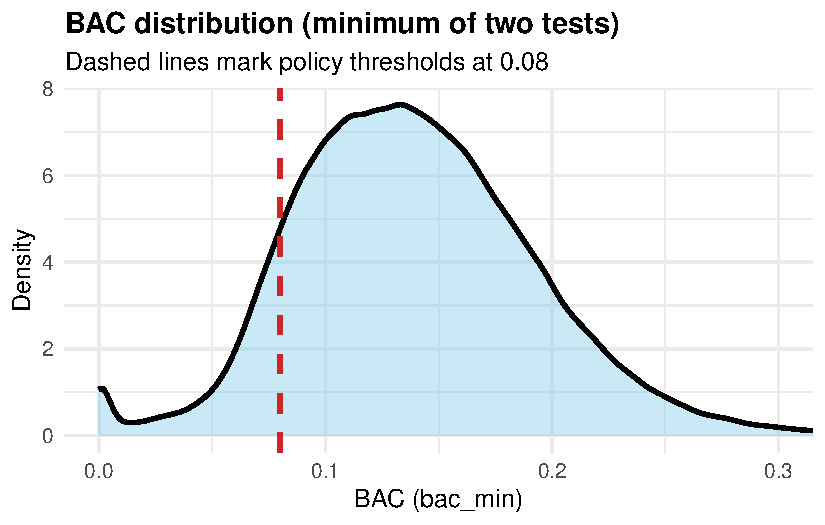
\includegraphics[keepaspectratio]{DTC_Group1-1_files/figure-pdf/bac-distribution-overall-1.pdf}}

\paragraph{4.3. BAC distribution near the 0.08
cutoff}\label{bac-distribution-near-the-0.08-cutoff}

To check for unusual ``bunching'' right at the legal threshold, we zoom
in on a narrow window around BAC = 0.08.

\begin{Shaded}
\begin{Highlighting}[]
\NormalTok{dwi\_008 }\OtherTok{\textless{}{-}}\NormalTok{ dwi }\SpecialCharTok{\%\textgreater{}\%} 
  \FunctionTok{filter}\NormalTok{(bac\_min }\SpecialCharTok{\textgreater{}=} \FloatTok{0.03}\NormalTok{, bac\_min }\SpecialCharTok{\textless{}=} \FloatTok{0.13}\NormalTok{)}

\FunctionTok{ggplot}\NormalTok{(dwi\_008, }\FunctionTok{aes}\NormalTok{(}\AttributeTok{x =}\NormalTok{ bac\_min)) }\SpecialCharTok{+}
  \FunctionTok{geom\_density}\NormalTok{(}\AttributeTok{fill =} \StringTok{"deepskyblue3"}\NormalTok{, }\AttributeTok{alpha =} \FloatTok{0.45}\NormalTok{, }\AttributeTok{linewidth =} \DecValTok{1}\NormalTok{) }\SpecialCharTok{+}
  \FunctionTok{geom\_vline}\NormalTok{(}\AttributeTok{xintercept =} \FloatTok{0.08}\NormalTok{, }\AttributeTok{linewidth =} \FloatTok{1.2}\NormalTok{, }\AttributeTok{linetype =} \StringTok{"dashed"}\NormalTok{, }\AttributeTok{colour =} \StringTok{"firebrick3"}\NormalTok{) }\SpecialCharTok{+}
  \FunctionTok{labs}\NormalTok{(}
    \AttributeTok{title =} \StringTok{"BAC distribution near the 0.08 cutoff"}\NormalTok{,}
    \AttributeTok{subtitle =} \StringTok{"Density plot for bac\_min in [0.03, 0.13]; dashed red line at 0.08"}\NormalTok{,}
    \AttributeTok{x =} \StringTok{"BAC (bac\_min)"}\NormalTok{,}
    \AttributeTok{y =} \StringTok{"Density"}
\NormalTok{  ) }\SpecialCharTok{+}
  \FunctionTok{theme\_minimal}\NormalTok{(}\AttributeTok{base\_size =} \DecValTok{12}\NormalTok{) }\SpecialCharTok{+}
  \FunctionTok{theme}\NormalTok{(}\AttributeTok{plot.title =} \FunctionTok{element\_text}\NormalTok{(}\AttributeTok{face =} \StringTok{"bold"}\NormalTok{))}
\end{Highlighting}
\end{Shaded}

\pandocbounded{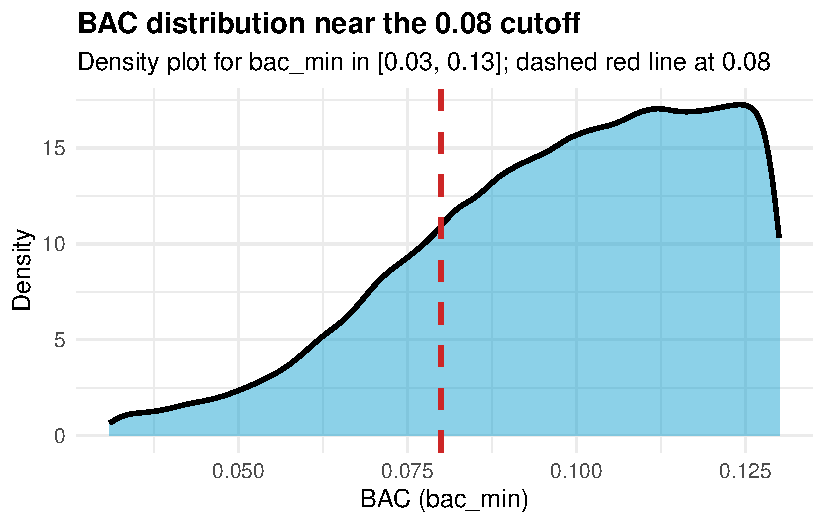
\includegraphics[keepaspectratio]{DTC_Group1-1_files/figure-pdf/bac-zoom-008-1.pdf}}

\paragraph{4.4. Baseline recidivism
rate}\label{baseline-recidivism-rate}

As a reference point, we compute the overall recidivism rate in the full
sample.

\begin{Shaded}
\begin{Highlighting}[]
\NormalTok{dwi }\SpecialCharTok{\%\textgreater{}\%}
  \FunctionTok{summarise}\NormalTok{(}
    \AttributeTok{n =} \FunctionTok{n}\NormalTok{(),}
    \AttributeTok{recidivism\_rate =} \FunctionTok{mean}\NormalTok{(recidivism, }\AttributeTok{na.rm =} \ConstantTok{TRUE}\NormalTok{)}
\NormalTok{  )}
\end{Highlighting}
\end{Shaded}

\begin{verbatim}
       n recidivism_rate
1 214558       0.1176325
\end{verbatim}

\paragraph{4.5. Missingness check}\label{missingness-check}

Before making any data-cleaning decisions, we report how much
`missingness' exists in the key analysis variables.

\begin{Shaded}
\begin{Highlighting}[]
\NormalTok{key\_vars }\OtherTok{\textless{}{-}} \FunctionTok{c}\NormalTok{(}\StringTok{"bac1"}\NormalTok{, }\StringTok{"bac2"}\NormalTok{, }\StringTok{"bac\_min"}\NormalTok{, }\StringTok{"recidivism"}\NormalTok{, }\StringTok{"male"}\NormalTok{, }\StringTok{"white"}\NormalTok{, }\StringTok{"aged"}\NormalTok{, }\StringTok{"acc"}\NormalTok{, }\StringTok{"year"}\NormalTok{)}

\NormalTok{dwi }\SpecialCharTok{\%\textgreater{}\%}
  \FunctionTok{summarise}\NormalTok{(}\FunctionTok{across}\NormalTok{(}\FunctionTok{all\_of}\NormalTok{(key\_vars), }\SpecialCharTok{\textasciitilde{}} \FunctionTok{mean}\NormalTok{(}\FunctionTok{is.na}\NormalTok{(.)))) }\SpecialCharTok{\%\textgreater{}\%}
  \FunctionTok{pivot\_longer}\NormalTok{(}\FunctionTok{everything}\NormalTok{(), }\AttributeTok{names\_to =} \StringTok{"variable"}\NormalTok{, }\AttributeTok{values\_to =} \StringTok{"missing\_share"}\NormalTok{) }\SpecialCharTok{\%\textgreater{}\%}
  \FunctionTok{arrange}\NormalTok{(}\FunctionTok{desc}\NormalTok{(missing\_share))}
\end{Highlighting}
\end{Shaded}

\begin{verbatim}
# A tibble: 9 x 2
  variable   missing_share
  <chr>              <dbl>
1 bac1                   0
2 bac2                   0
3 bac_min                0
4 recidivism             0
5 male                   0
6 white                  0
7 aged                   0
8 acc                    0
9 year                   0
\end{verbatim}

\paragraph{4.6. Quick near-cutoff
comparison}\label{quick-near-cutoff-comparison}

As an initial descriptive check, we compare observations just below vs
just above each cutoff within a narrow window (±0.02 BAC). This is not
the final regression discontinuity estimate, but it provides an early
sense of whether outcomes and co-variates look similar near the
threshold.

\begin{Shaded}
\begin{Highlighting}[]
\NormalTok{w }\OtherTok{\textless{}{-}} \FloatTok{0.02}  \CommentTok{\# window size (±0.02)}

\NormalTok{summary\_near }\OtherTok{\textless{}{-}} \ControlFlowTok{function}\NormalTok{(cutoff) \{}
\NormalTok{  dwi }\SpecialCharTok{\%\textgreater{}\%}
    \FunctionTok{filter}\NormalTok{(bac\_min }\SpecialCharTok{\textgreater{}=}\NormalTok{ cutoff }\SpecialCharTok{{-}}\NormalTok{ w, bac\_min }\SpecialCharTok{\textless{}=}\NormalTok{ cutoff }\SpecialCharTok{+}\NormalTok{ w) }\SpecialCharTok{\%\textgreater{}\%}
    \FunctionTok{mutate}\NormalTok{(}\AttributeTok{above =} \FunctionTok{as.integer}\NormalTok{(bac\_min }\SpecialCharTok{\textgreater{}=}\NormalTok{ cutoff)) }\SpecialCharTok{\%\textgreater{}\%}
    \FunctionTok{group\_by}\NormalTok{(above) }\SpecialCharTok{\%\textgreater{}\%}
    \FunctionTok{summarise}\NormalTok{(}
      \AttributeTok{n =} \FunctionTok{n}\NormalTok{(),}
      \AttributeTok{recid\_rate =} \FunctionTok{mean}\NormalTok{(recidivism),}
      \AttributeTok{male\_share =} \FunctionTok{mean}\NormalTok{(male),}
      \AttributeTok{white\_share =} \FunctionTok{mean}\NormalTok{(white),}
      \AttributeTok{mean\_age =} \FunctionTok{mean}\NormalTok{(aged),}
      \AttributeTok{acc\_share =} \FunctionTok{mean}\NormalTok{(acc),}
      \AttributeTok{.groups =} \StringTok{"drop"}
\NormalTok{    ) }\SpecialCharTok{\%\textgreater{}\%}
    \FunctionTok{mutate}\NormalTok{(}\AttributeTok{cutoff =}\NormalTok{ cutoff) }\SpecialCharTok{\%\textgreater{}\%}
    \FunctionTok{relocate}\NormalTok{(cutoff, above)}
\NormalTok{\}}

\FunctionTok{bind\_rows}\NormalTok{(}
  \FunctionTok{summary\_near}\NormalTok{(}\FloatTok{0.08}\NormalTok{),}
\NormalTok{) }\SpecialCharTok{\%\textgreater{}\%}
  \FunctionTok{arrange}\NormalTok{(cutoff, above)}
\end{Highlighting}
\end{Shaded}

\begin{verbatim}
# A tibble: 2 x 8
  cutoff above     n recid_rate male_share white_share mean_age acc_share
   <dbl> <int> <int>      <dbl>      <dbl>       <dbl>    <dbl>     <dbl>
1   0.08     0 14584     0.115       0.784       0.846     34.5    0.0902
2   0.08     1 25790     0.0989      0.792       0.852     33.9    0.0899
\end{verbatim}

At 0.08, recidivism is lower just above the cutoff (≈ 0.0989) than just
below (≈ 0.1147).

\paragraph{4.7. Interim takeaways from initial
exploration}\label{interim-takeaways-from-initial-exploration}

At this stage, we have, (i) created the running variable for the
regression discontinuity design (\texttt{bac\_min}, defined as the
minimum of the two BAC tests), (ii) checked basic data quality.

The distribution of \texttt{bac\_min} looks smooth overall and around
the policy cutoff (0.08) based on the density plots. Missingness is
effectively zero in the key variables used in later analysis, so no
sample exclusions are required for missing data.

As an initial descriptive comparison within ±0.02 of each cutoff,
recidivism appears lower just above 0.08 than just below. These
comparisons are descriptive and do not yet isolate the causal effect;
they mainly motivate the formal RDD analysis in the next stage.

\paragraph{4.8. Difference summary
table}\label{difference-summary-table}

\begin{Shaded}
\begin{Highlighting}[]
\NormalTok{near\_tbl }\OtherTok{\textless{}{-}} \FunctionTok{bind\_rows}\NormalTok{(}
  \FunctionTok{summary\_near}\NormalTok{(}\FloatTok{0.08}\NormalTok{),}
\NormalTok{)}

\NormalTok{near\_tbl }\SpecialCharTok{\%\textgreater{}\%}
  \FunctionTok{group\_by}\NormalTok{(cutoff) }\SpecialCharTok{\%\textgreater{}\%}
  \FunctionTok{summarise}\NormalTok{(}
    \AttributeTok{diff\_recid =}\NormalTok{ recid\_rate[above }\SpecialCharTok{==} \DecValTok{1}\NormalTok{] }\SpecialCharTok{{-}}\NormalTok{ recid\_rate[above }\SpecialCharTok{==} \DecValTok{0}\NormalTok{],}
    \AttributeTok{diff\_male  =}\NormalTok{ male\_share[above }\SpecialCharTok{==} \DecValTok{1}\NormalTok{] }\SpecialCharTok{{-}}\NormalTok{ male\_share[above }\SpecialCharTok{==} \DecValTok{0}\NormalTok{],}
    \AttributeTok{diff\_white =}\NormalTok{ white\_share[above }\SpecialCharTok{==} \DecValTok{1}\NormalTok{] }\SpecialCharTok{{-}}\NormalTok{ white\_share[above }\SpecialCharTok{==} \DecValTok{0}\NormalTok{],}
    \AttributeTok{diff\_age   =}\NormalTok{ mean\_age[above }\SpecialCharTok{==} \DecValTok{1}\NormalTok{] }\SpecialCharTok{{-}}\NormalTok{ mean\_age[above }\SpecialCharTok{==} \DecValTok{0}\NormalTok{],}
    \AttributeTok{diff\_acc   =}\NormalTok{ acc\_share[above }\SpecialCharTok{==} \DecValTok{1}\NormalTok{] }\SpecialCharTok{{-}}\NormalTok{ acc\_share[above }\SpecialCharTok{==} \DecValTok{0}\NormalTok{],}
    \AttributeTok{.groups =} \StringTok{"drop"}
\NormalTok{  )}
\end{Highlighting}
\end{Shaded}

\begin{verbatim}
# A tibble: 1 x 6
  cutoff diff_recid diff_male diff_white diff_age  diff_acc
   <dbl>      <dbl>     <dbl>      <dbl>    <dbl>     <dbl>
1   0.08    -0.0158   0.00735    0.00596   -0.606 -0.000356
\end{verbatim}

\subsection{\texorpdfstring{\textbf{5. DAG: Visualizing the causal
relationship}}{5. DAG: Visualizing the causal relationship}}\label{dag-visualizing-the-causal-relationship}

\begin{figure}[H]

{\centering 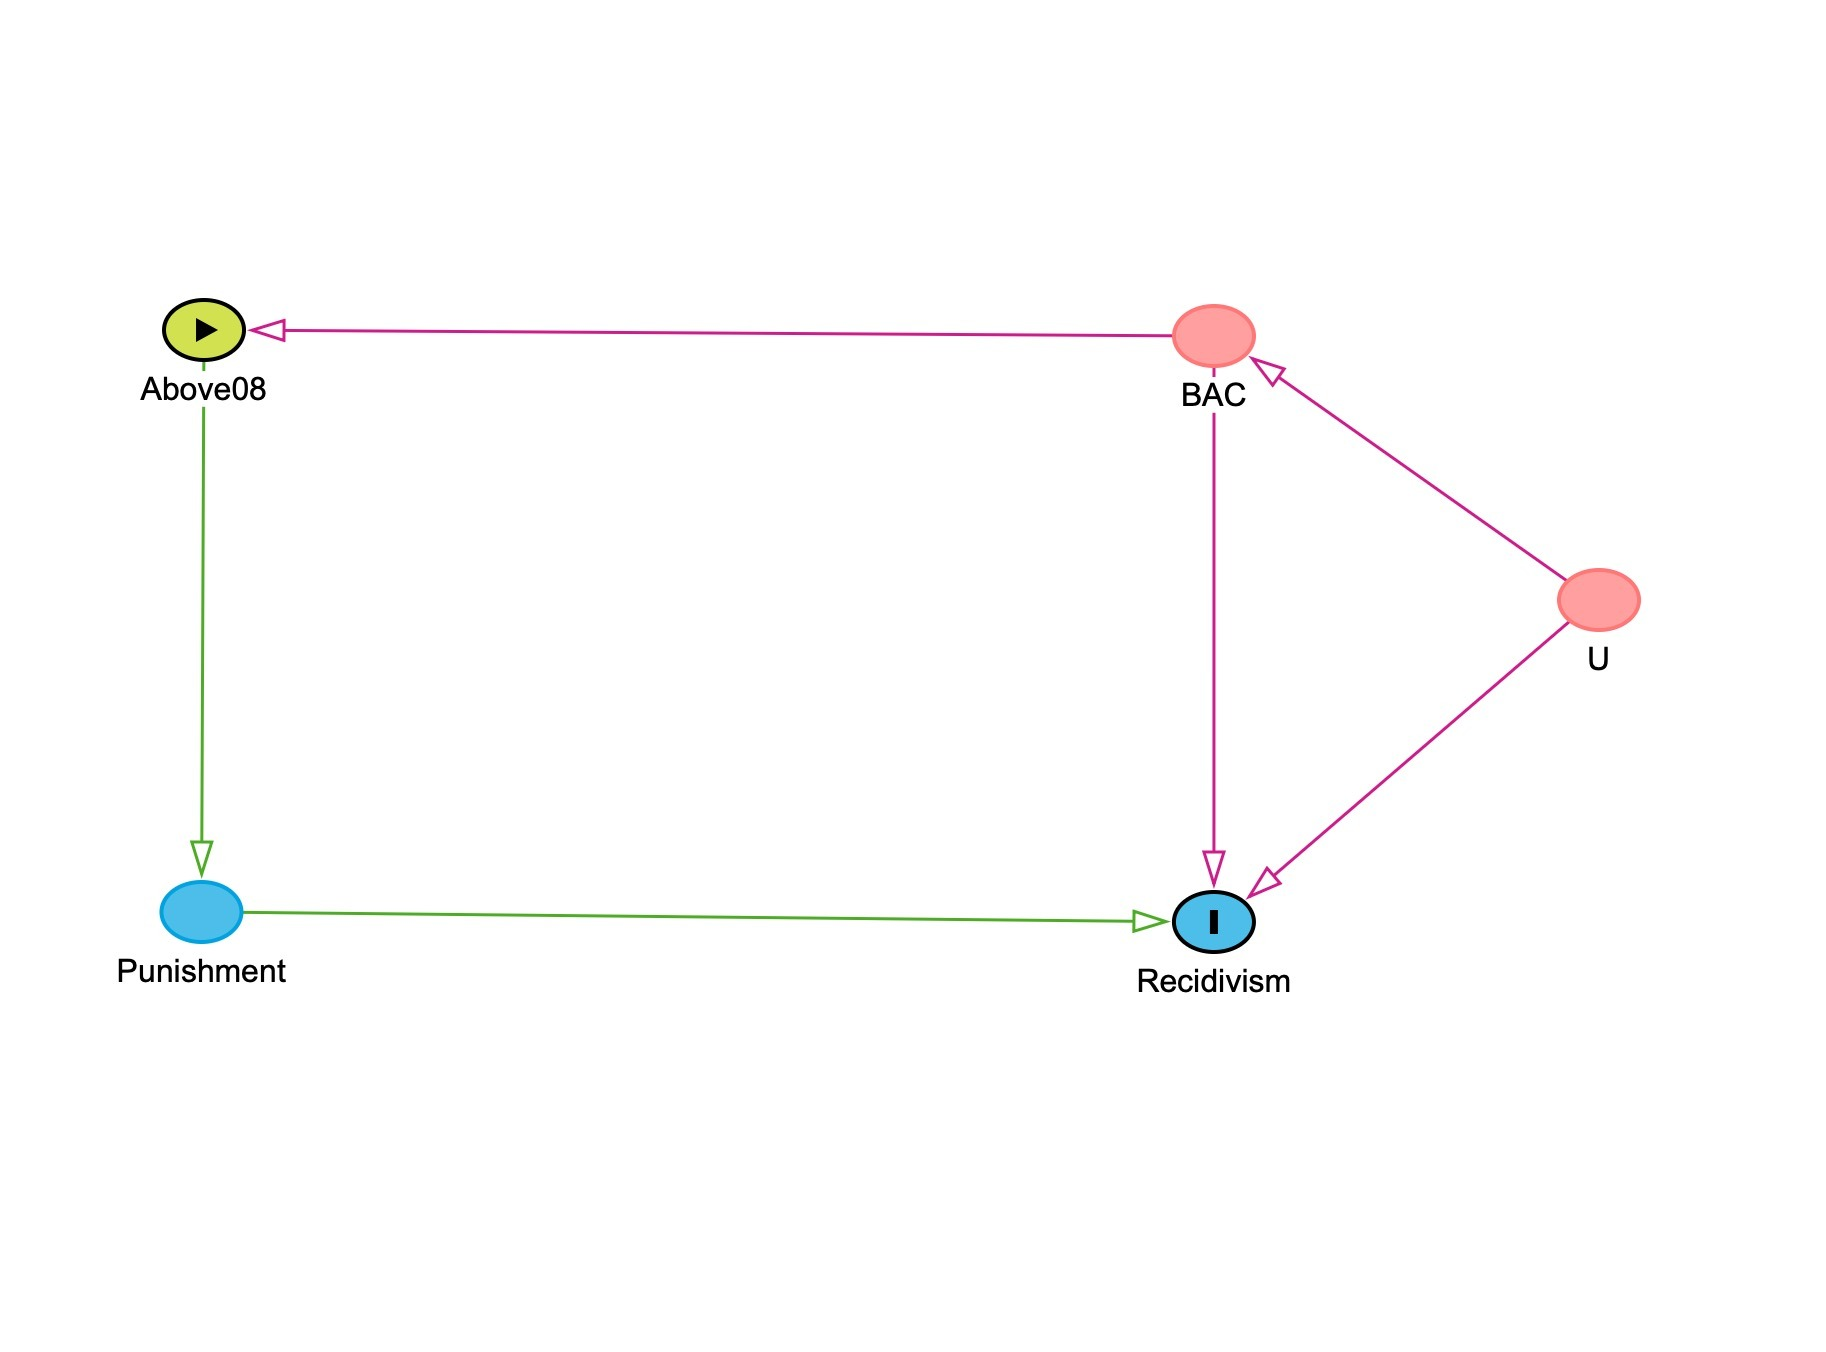
\includegraphics[width=7.64583in,height=\textheight,keepaspectratio]{dagitty-model.jpeg}

}

\caption{\emph{Figure. 6. Simplified DAG showing the Causal logic}}

\end{figure}%

Figure presents the causal logic behind our regression discontinuity
design. BAC is the running variable, and the node BAC ≥ 0.08~represents
the legal assignment rule that determines whether a driver is exposed to
harsher DUI punishment. That punishment is the treatment mechanism
through which crossing the threshold may affect future recidivism. The
diagram also includes U, which captures unobserved driver
characteristics, such as alcohol misuse or alcoholism, impulsiveness, or
risk tolerance, that may influence both BAC and the likelihood of
reoffending. These unobserved factors create a backdoor path that would
bias a simple comparison of drivers with higher and lower BAC levels. By
focusing on drivers just below and just above the 0.08 cutoff, the RD
design uses the policy cutoff to isolate the local causal effect of
harsher punishment on recidivism.

\subsection{5.1. Causal Logic}\label{causal-logic}

Building on the causal structure shown in Figure 6, the key empirical
challenge is to isolate the effect of harsher DUI punishment from the
characteristics of the drivers who receive it. Drivers with higher BAC
levels are more likely to face tougher penalties, but they may also
differ in less visible ways, such as impulsiveness, alcohol misuse, or a
greater willingness to take risks, that independently increase the
likelihood of reoffending. For that reason, a simple comparison between
drivers with lower and higher BAC levels would confound the effect of
punishment with the effect of those underlying differences.

The 0.08 BAC cutoff helps address this problem. Because Washington
State's DUI penalties increase sharply at that threshold, drivers just
below and just above 0.08 should be very similar, while only those above
the cutoff receive harsher punishment. This is what makes the setting
well suited to a regression discontinuity design: by comparing drivers
very close to the threshold, we can use the policy rule as a natural
experiment to estimate the local effect of harsher punishment on future
recidivism. In the next step, we will be assess whether the assumptions
required for that design are supported by the data.

\subsection{6. Identification Assumptions and Supporting
Checks}\label{identification-assumptions-and-supporting-checks}

\subsection{i. Checking Data for
Lumping}\label{i.-checking-data-for-lumping}

Now that the data are prepared and the causal logic is clear, the next
step is to test whether the key assumptions of the regression
discontinuity design are plausible in this setting. Before estimating
the treatment effect at the 0.08 BAC cutoff, we need to check that
drivers are not systematically sorting to one side of the threshold or
the other. We assess this by examining the distribution of the running
variable near the cutoff with a lumping test. We also need to verify
that drivers just below and just above 0.08 look similar on
predetermined characteristics. We assess that by estimating placebo
regressions using variables that should not jump at the threshold.

A useful first check is whether there is any manipulation in the running
variable around 0.08. To examine this, we graph the BAC distribution
using bins and look for any unusual break or bunching in the number of
observations right at the cutoff.

\begin{Shaded}
\begin{Highlighting}[]
\CommentTok{\#Check lumping at the 0.08 cutoff}
\NormalTok{dwi\_bin\_count }\OtherTok{\textless{}{-}}\NormalTok{ dwi }\SpecialCharTok{\%\textgreater{}\%}
  \FunctionTok{filter}\NormalTok{(bac\_min }\SpecialCharTok{\textgreater{}=} \FloatTok{0.03}\NormalTok{, bac\_min }\SpecialCharTok{\textless{}=} \FloatTok{0.13}\NormalTok{) }\SpecialCharTok{\%\textgreater{}\%}
  \FunctionTok{mutate}\NormalTok{(}\AttributeTok{bac\_bins =} \FunctionTok{cut}\NormalTok{(bac\_min, }\AttributeTok{breaks =} \DecValTok{3}\SpecialCharTok{:}\DecValTok{13}\SpecialCharTok{/}\DecValTok{100}\NormalTok{)) }\SpecialCharTok{\%\textgreater{}\%}
  \FunctionTok{group\_by}\NormalTok{(bac\_bins) }\SpecialCharTok{\%\textgreater{}\%}
  \FunctionTok{count}\NormalTok{()}

\CommentTok{\#Create plot to visualize the data}
\FunctionTok{ggplot}\NormalTok{(dwi\_bin\_count, }\FunctionTok{aes}\NormalTok{(}\AttributeTok{x =}\NormalTok{ bac\_bins, }\AttributeTok{y =}\NormalTok{ n)) }\SpecialCharTok{+}
  \FunctionTok{geom\_col}\NormalTok{() }\SpecialCharTok{+}
  \FunctionTok{geom\_vline}\NormalTok{(}\AttributeTok{xintercept =} \FloatTok{5.5}\NormalTok{,}
             \AttributeTok{color =} \StringTok{"red"}\NormalTok{, }\AttributeTok{linetype =} \StringTok{"dashed"}\NormalTok{) }\SpecialCharTok{+}
  \FunctionTok{labs}\NormalTok{(}\AttributeTok{title =} \StringTok{"Observation counts near 0.08 BAC cutoff"}\NormalTok{,}
       \AttributeTok{x =} \StringTok{"BAC bin"}\NormalTok{, }\AttributeTok{y =} \StringTok{"Count"}\NormalTok{) }\SpecialCharTok{+}
  \FunctionTok{theme\_minimal}\NormalTok{() }\SpecialCharTok{+}
  \FunctionTok{theme}\NormalTok{(}\AttributeTok{axis.text.x =} \FunctionTok{element\_text}\NormalTok{(}\AttributeTok{angle =} \DecValTok{45}\NormalTok{, }\AttributeTok{hjust =} \DecValTok{1}\NormalTok{))}
\end{Highlighting}
\end{Shaded}

\pandocbounded{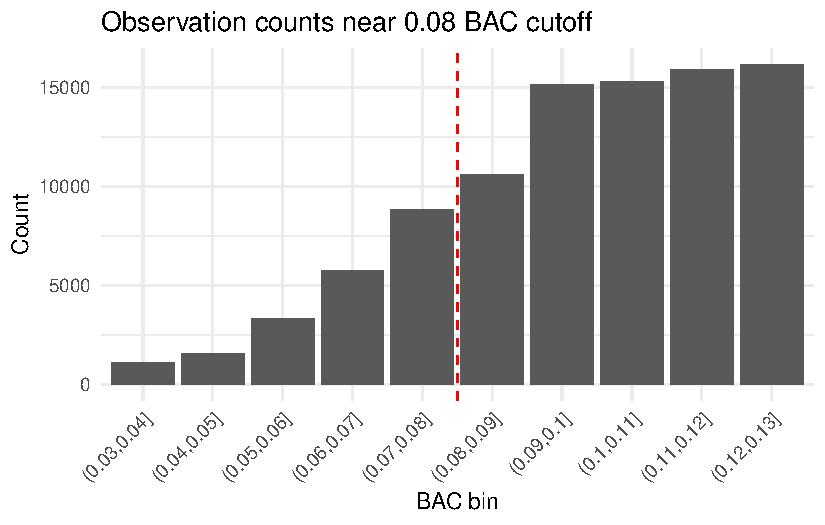
\includegraphics[keepaspectratio]{DTC_Group1-1_files/figure-pdf/unnamed-chunk-5-1.pdf}}

\begin{verbatim}
\end{verbatim}

We use this visual check is used to assess whether there is manipulation
of the running variable, a key assumption for a valid regression
discontinuity design. If drivers or law enforcement were systematically
influencing BAC readings to fall on one side of the threshold, we would
expect to observe a sharp spike or drop in the number of observations
immediately below or above the cutoff. Instead, the distribution appears
smooth, with no noticeable bunching just below 0.08. This suggests that
drivers are not sorting around the threshold and that BAC readings near
the cutoff are plausibly random. Because the distribution remains
continuous at the threshold, the identifying assumption of the RD design
appears reasonable, allowing us to proceed with placebo

\subsection{6.ii. The Placebo Tests}\label{ii.-the-placebo-tests}

Our placebo tests evaluate whether the observations just below and just
above the 0.08 BAC cutoff are truly comparable. We run these tests
because a valid regression discontinuity design requires that the cutoff
changes only the treatment intensity, in this case, harsher punishment,
and not other underlying characteristics of the drivers. To check this,
we re-estimate the RD specification using predetermined variables such
as male, white, aged, and acc as outcomes instead of recidivism. If the
design is credible, we should not observe a discontinuous jump at the
cutoff for any of these variables. A significant jump would suggest that
drivers on either side of 0.08 differ in ways other than punishment,
which would weaken the validity of the comparison. Because our analysis
focuses on the instructor-approved~0.08 threshold, we perform these
placebo checks only at that cutoff.

\begin{Shaded}
\begin{Highlighting}[]
\CommentTok{\#Create centered variable for BAC at 0.08 cutoff}
\NormalTok{dwi }\OtherTok{\textless{}{-}}\NormalTok{ dwi }\SpecialCharTok{\%\textgreater{}\%}
  \FunctionTok{mutate}\NormalTok{(}\AttributeTok{bac\_centered\_08 =}\NormalTok{ bac\_min }\SpecialCharTok{{-}} \FloatTok{0.08}\NormalTok{)}

\CommentTok{\# Run placebo regressions at the 0.08 cutoff}
\NormalTok{p1 }\OtherTok{\textless{}{-}} \FunctionTok{feols}\NormalTok{(male  }\SpecialCharTok{\textasciitilde{}}\NormalTok{ above\_08 }\SpecialCharTok{*}\NormalTok{ bac\_centered\_08,}
            \AttributeTok{data =}\NormalTok{ dwi }\SpecialCharTok{\%\textgreater{}\%} \FunctionTok{filter}\NormalTok{(}\FunctionTok{abs}\NormalTok{(bac\_centered\_08) }\SpecialCharTok{\textless{}} \FloatTok{0.05}\NormalTok{),}
            \AttributeTok{vcov =} \StringTok{"hetero"}\NormalTok{)}

\NormalTok{p2 }\OtherTok{\textless{}{-}} \FunctionTok{feols}\NormalTok{(white }\SpecialCharTok{\textasciitilde{}}\NormalTok{ above\_08 }\SpecialCharTok{*}\NormalTok{ bac\_centered\_08,}
            \AttributeTok{data =}\NormalTok{ dwi }\SpecialCharTok{\%\textgreater{}\%} \FunctionTok{filter}\NormalTok{(}\FunctionTok{abs}\NormalTok{(bac\_centered\_08) }\SpecialCharTok{\textless{}} \FloatTok{0.05}\NormalTok{),}
            \AttributeTok{vcov =} \StringTok{"hetero"}\NormalTok{)}

\NormalTok{p3 }\OtherTok{\textless{}{-}} \FunctionTok{feols}\NormalTok{(aged  }\SpecialCharTok{\textasciitilde{}}\NormalTok{ above\_08 }\SpecialCharTok{*}\NormalTok{ bac\_centered\_08,}
            \AttributeTok{data =}\NormalTok{ dwi }\SpecialCharTok{\%\textgreater{}\%} \FunctionTok{filter}\NormalTok{(}\FunctionTok{abs}\NormalTok{(bac\_centered\_08) }\SpecialCharTok{\textless{}} \FloatTok{0.05}\NormalTok{),}
            \AttributeTok{vcov =} \StringTok{"hetero"}\NormalTok{)}

\NormalTok{p4 }\OtherTok{\textless{}{-}} \FunctionTok{feols}\NormalTok{(acc   }\SpecialCharTok{\textasciitilde{}}\NormalTok{ above\_08 }\SpecialCharTok{*}\NormalTok{ bac\_centered\_08,}
            \AttributeTok{data =}\NormalTok{ dwi }\SpecialCharTok{\%\textgreater{}\%} \FunctionTok{filter}\NormalTok{(}\FunctionTok{abs}\NormalTok{(bac\_centered\_08) }\SpecialCharTok{\textless{}} \FloatTok{0.05}\NormalTok{),}
            \AttributeTok{vcov =} \StringTok{"hetero"}\NormalTok{)}

\FunctionTok{etable}\NormalTok{(p1, p2, p3, p4)}
\end{Highlighting}
\end{Shaded}

\begin{verbatim}
                                           p1                 p2
Dependent Var.:                          male              white
                                                                
Constant                   0.7853*** (0.0045) 0.8478*** (0.0039)
above_08                      0.0057 (0.0055)    0.0038 (0.0049)
bac_centered_08              -0.1752 (0.2330)    0.0552 (0.2052)
above_08 x bac_centered_08    0.2947 (0.2575)    0.0488 (0.2264)
__________________________ __________________ __________________
S.E. type                  Heteroskedas.-rob. Heteroskedas.-rob.
Observations                           92,158             92,158
R2                                    6.05e-5            8.86e-5
Adj. R2                                2.8e-5             5.6e-5

                                          p3                 p4
Dependent Var.:                         aged                acc
                                                               
Constant                   33.92*** (0.1297) 0.0825*** (0.0031)
above_08                    -0.1647 (0.1596)   -0.0022 (0.0039)
bac_centered_08            -66.52*** (7.012) -1.044*** (0.1772)
above_08 x bac_centered_08  73.75*** (7.666)  1.901*** (0.1954)
__________________________ _________________ __________________
S.E. type                  Heteroskeda.-rob. Heteroskedas.-rob.
Observations                          92,158             92,158
R2                                   0.00232            0.00163
Adj. R2                              0.00229            0.00160
---
Signif. codes: 0 '***' 0.001 '**' 0.01 '*' 0.05 '.' 0.1 ' ' 1
\end{verbatim}

The placebo regression results provide a useful check on whether drivers
just below and just above the 0.08 BAC cutoff are comparable. In these
models, we replace recidivism with predetermined characteristics, sex,
race, age, and accident involvement, and estimate the same regression
discontinuity specification used in the main analysis. The coefficient
of interest is the indicator for being above the cutoff, since it
captures any discrete jump at the threshold. Across these regressions,
that coefficient is small and statistically insignificant in every case,
suggesting that these observable characteristics do not change abruptly
at 0.08. This pattern is consistent with the idea that drivers on either
side of the legal threshold are similar in observable ways, which
supports the credibility of the regression discontinuity design. We
report heteroskedasticity-robust standard errors in the placebo
regressions for consistency with the main analysis and because the
variance of the error term may differ across observations.

\subsection{7. Regression Discontinuity
Specification}\label{regression-discontinuity-specification}

\begin{enumerate}
\def\labelenumi{\arabic{enumi}.}
\setcounter{enumi}{6}
\tightlist
\item
  \textbf{i. The working equation}
\end{enumerate}

\[
\text{Recidivism}_i = \beta_0 + \beta_1 \text{Above08}_i + \beta_2 (BAC_i - 0.08) + \beta_3 \big[\text{Above08}_i \times (BAC_i - 0.08)\big] + \varepsilon_i
\]

To estimate the effect of harsher punishment at the legal threshold, we
use a local linear regression discontinuity specification centered at
BAC = 0.08. In this model,~\texttt{Above08} indicates whether a driver
falls at or above the legal cutoff, while the centered BAC term measures
distance from the threshold. The interaction term allows the
relationship between BAC and recidivism to differ on either side of the
cutoff. The coefficient of primary interest is B1\hspace{0pt}, which
captures the discontinuous jump in recidivism at \textbf{0.08} and
represents the local effect of crossing the legal BAC limit.

\subsection{8. Main Regression Discontinuity
Models}\label{main-regression-discontinuity-models}

Now that we have checked the key assumptions in our data set, we proceed
with the main analysis. We want to determine whether crossing the BAC
threshold, and receiving a harsh punishment, causes a decrease in
recidivism. Firstly, we center the running variable around each cutoff
point, creating a treatment indicator for being above the threshold and
then interact these two variables. The coefficient on the treatment
indicator shows the jump in recidivism at the cutoff, which is our
estimate of the effect of a harsher punishment. We then run three
different variations for each cutoff: 1) a wider window of 0.05, 2) a
narrower window of 0.02, and 3) a wide window with our additional
variables added as controls. We then compare the results among these
three variations to see if our results are stable.

\begin{enumerate}
\def\labelenumi{\arabic{enumi}.}
\setcounter{enumi}{6}
\tightlist
\item
  \textbf{i. Main RD Estimate at the 0.08 BAC Cutoff (±0.05 Window)}
\end{enumerate}

\begin{Shaded}
\begin{Highlighting}[]
\NormalTok{r1 }\OtherTok{\textless{}{-}} \FunctionTok{feols}\NormalTok{(}
\NormalTok{  recidivism }\SpecialCharTok{\textasciitilde{}}\NormalTok{ above\_08 }\SpecialCharTok{*}\NormalTok{ bac\_centered\_08,}
  \AttributeTok{data =}\NormalTok{ dwi }\SpecialCharTok{\%\textgreater{}\%} \FunctionTok{filter}\NormalTok{(}\FunctionTok{abs}\NormalTok{(bac\_centered\_08) }\SpecialCharTok{\textless{}} \FloatTok{0.05}\NormalTok{),}
  \AttributeTok{vcov =} \StringTok{"hetero"}
\NormalTok{)}

\FunctionTok{etable}\NormalTok{(r1)}
\end{Highlighting}
\end{Shaded}

\begin{verbatim}
                                            r1
Dependent Var.:                     recidivism
                                              
Constant                    0.1123*** (0.0034)
above_08                   -0.0188*** (0.0042)
bac_centered_08               -0.2613 (0.1818)
above_08 x bac_centered_08  0.6904*** (0.1998)
__________________________ ___________________
S.E. type                  Heteroskedast.-rob.
Observations                            92,158
R2                                     0.00054
Adj. R2                                0.00051
---
Signif. codes: 0 '***' 0.001 '**' 0.01 '*' 0.05 '.' 0.1 ' ' 1
\end{verbatim}

Regression table 1.

We estimate a local linear regression discontinuity model within a ±0.05
window around the 0.08 BAC cutoff to compare drivers who are closest to
the legal threshold. This choice is justified because RD relies on local
comparisons, where observations just below and just above the cutoff are
most plausibly similar except for the harsher punishment triggered at
0.08. The interaction between above\_08 and bac\_centered\_08 allows the
BAC--recidivism relationship to differ on either side of the threshold
while identifying the jump at the cutoff. The coefficient on above\_08
is -0.0188 and statistically significant, indicating that drivers just
above 0.08 have an estimated recidivism rate about 1.9 percentage points
lower than comparable drivers just below the cutoff.

\begin{enumerate}
\def\labelenumi{\arabic{enumi}.}
\setcounter{enumi}{6}
\tightlist
\item
  \textbf{ii. Robustness Check: Narrower Bandwidth (±0.02)}
\end{enumerate}

\begin{Shaded}
\begin{Highlighting}[]
\NormalTok{r2 }\OtherTok{\textless{}{-}} \FunctionTok{feols}\NormalTok{(recidivism }\SpecialCharTok{\textasciitilde{}}\NormalTok{ above\_08 }\SpecialCharTok{*}\NormalTok{ bac\_centered\_08,}
            \AttributeTok{data =}\NormalTok{ dwi }\SpecialCharTok{\%\textgreater{}\%} \FunctionTok{filter}\NormalTok{(}\FunctionTok{abs}\NormalTok{(bac\_centered\_08) }\SpecialCharTok{\textless{}} \FloatTok{0.02}\NormalTok{), }\AttributeTok{vcov =}\StringTok{"hetero"}\NormalTok{)}
\FunctionTok{etable}\NormalTok{(r2)}
\end{Highlighting}
\end{Shaded}

\begin{verbatim}
                                           r2
Dependent Var.:                    recidivism
                                             
Constant                   0.1074*** (0.0046)
above_08                    -0.0133* (0.0061)
bac_centered_08             -0.8974. (0.4699)
above_08 x bac_centered_08    1.262* (0.5847)
__________________________ __________________
S.E. type                  Heteroskedas.-rob.
Observations                           38,962
R2                                    0.00083
Adj. R2                               0.00075
---
Signif. codes: 0 '***' 0.001 '**' 0.01 '*' 0.05 '.' 0.1 ' ' 1
\end{verbatim}

We use a bandwidth of ±0.02 around the 0.08 cutoff, meaning the
estimation sample includes drivers with BAC values between~0.06 and
0.10. This narrower specification serves as a robustness check by
focusing on observations even closer to the threshold, where drivers
just below and just above 0.08 are most plausibly comparable. In this
model, the coefficient on~\texttt{above\_08} is −0.0133 and remains
statistically significant at the 5 percent level. This implies that
drivers just above the legal cutoff have an estimated recidivism rate
about 1.3 percentage points lower than those just below it, reinforcing
the main deterrence result from the wider bandwidth specification.

\begin{enumerate}
\def\labelenumi{\arabic{enumi}.}
\setcounter{enumi}{6}
\tightlist
\item
  \textbf{iii. Robustness Check: RD Estimate with Demographic Controls}
\end{enumerate}

\begin{Shaded}
\begin{Highlighting}[]
\NormalTok{r3 }\OtherTok{\textless{}{-}} \FunctionTok{feols}\NormalTok{(recidivism }\SpecialCharTok{\textasciitilde{}}\NormalTok{ above\_08 }\SpecialCharTok{*}\NormalTok{ bac\_centered\_08 }\SpecialCharTok{+}\NormalTok{ male }\SpecialCharTok{+}\NormalTok{ white }\SpecialCharTok{+}\NormalTok{ aged,}
            \AttributeTok{data =}\NormalTok{ dwi }\SpecialCharTok{\%\textgreater{}\%} \FunctionTok{filter}\NormalTok{(}\FunctionTok{abs}\NormalTok{(bac\_centered\_08) }\SpecialCharTok{\textless{}} \FloatTok{0.05}\NormalTok{), }\AttributeTok{vcov =} \StringTok{"hetero"}\NormalTok{)}
\FunctionTok{etable}\NormalTok{(r3)}
\end{Highlighting}
\end{Shaded}

\begin{verbatim}
                                             r3
Dependent Var.:                      recidivism
                                               
Constant                     0.1019*** (0.0052)
above_08                    -0.0192*** (0.0042)
bac_centered_08               -0.3129. (0.1815)
male                         0.0331*** (0.0023)
white                        0.0157*** (0.0028)
aged                       -0.0009*** (8.39e-5)
above_08 x bac_centered_08   0.7427*** (0.1995)
__________________________ ____________________
S.E. type                  Heteroskedasti.-rob.
Observations                             92,158
R2                                      0.00360
Adj. R2                                 0.00353
---
Signif. codes: 0 '***' 0.001 '**' 0.01 '*' 0.05 '.' 0.1 ' ' 1
\end{verbatim}

The above regression adds male, white, and age as controls within the
same ±0.05 bandwidth around the 0.08 cutoff. In an RD design, these
controls are not needed for identification if the continuity assumption
holds, but they are useful as a robustness check because they can
improve precision and show whether the estimated jump is sensitive to
modest covariate adjustment. The coefficient on \texttt{above\_08} is
-0.0192, nearly identical to the baseline estimate of -0.0188. This
stability suggests that the main result is not being driven by
observable demographic differences, strengthening the interpretation
that crossing 0.08 reduces recidivism locally.

\subsection{8. Results and
Interpretation}\label{results-and-interpretation}

\begin{enumerate}
\def\labelenumi{\arabic{enumi}.}
\setcounter{enumi}{7}
\tightlist
\item
  \textbf{i. RD plot of recidivism around 0.08 cutoff.}
\end{enumerate}

\begin{Shaded}
\begin{Highlighting}[]
\CommentTok{\#| label: rd{-}plot{-}recidivism}

\FunctionTok{library}\NormalTok{(ggplot2)}
\FunctionTok{library}\NormalTok{(dplyr)}

\NormalTok{dwi }\SpecialCharTok{\%\textgreater{}\%}
  \FunctionTok{filter}\NormalTok{(}\FunctionTok{abs}\NormalTok{(bac\_centered\_08) }\SpecialCharTok{\textless{}} \FloatTok{0.05}\NormalTok{) }\SpecialCharTok{\%\textgreater{}\%}   \CommentTok{\# same bandwidth as main regression}
  \FunctionTok{ggplot}\NormalTok{(}\FunctionTok{aes}\NormalTok{(}\AttributeTok{x =}\NormalTok{ bac\_centered\_08, }\AttributeTok{y =}\NormalTok{ recidivism)) }\SpecialCharTok{+}

  \CommentTok{\# binned means}
  \FunctionTok{stat\_summary\_bin}\NormalTok{(}
    \AttributeTok{bins =} \DecValTok{30}\NormalTok{,}
    \AttributeTok{fun =}\NormalTok{ mean,}
    \AttributeTok{geom =} \StringTok{"point"}\NormalTok{,}
    \AttributeTok{color =} \StringTok{"black"}
\NormalTok{  ) }\SpecialCharTok{+}

  \CommentTok{\# fitted line left of cutoff}
  \FunctionTok{geom\_smooth}\NormalTok{(}
    \AttributeTok{data =}\NormalTok{ dwi }\SpecialCharTok{\%\textgreater{}\%} \FunctionTok{filter}\NormalTok{(bac\_centered\_08 }\SpecialCharTok{\textless{}} \DecValTok{0} \SpecialCharTok{\&} \FunctionTok{abs}\NormalTok{(bac\_centered\_08) }\SpecialCharTok{\textless{}} \FloatTok{0.05}\NormalTok{),}
    \AttributeTok{method =} \StringTok{"lm"}\NormalTok{,}
    \AttributeTok{se =} \ConstantTok{FALSE}\NormalTok{,}
    \AttributeTok{color =} \StringTok{"steelblue"}
\NormalTok{  ) }\SpecialCharTok{+}

  \CommentTok{\# fitted line right of cutoff}
  \FunctionTok{geom\_smooth}\NormalTok{(}
    \AttributeTok{data =}\NormalTok{ dwi }\SpecialCharTok{\%\textgreater{}\%} \FunctionTok{filter}\NormalTok{(bac\_centered\_08 }\SpecialCharTok{\textgreater{}=} \DecValTok{0} \SpecialCharTok{\&} \FunctionTok{abs}\NormalTok{(bac\_centered\_08) }\SpecialCharTok{\textless{}} \FloatTok{0.05}\NormalTok{),}
    \AttributeTok{method =} \StringTok{"lm"}\NormalTok{,}
    \AttributeTok{se =} \ConstantTok{FALSE}\NormalTok{,}
    \AttributeTok{color =} \StringTok{"red"}
\NormalTok{  ) }\SpecialCharTok{+}

  \FunctionTok{geom\_vline}\NormalTok{(}\AttributeTok{xintercept =} \DecValTok{0}\NormalTok{, }\AttributeTok{linetype =} \StringTok{"dashed"}\NormalTok{) }\SpecialCharTok{+}

  \FunctionTok{labs}\NormalTok{(}
    \AttributeTok{title =} \StringTok{"Recidivism Around the 0.08 BAC Cutoff"}\NormalTok{,}
    \AttributeTok{x =} \StringTok{"BAC centered at 0.08"}\NormalTok{,}
    \AttributeTok{y =} \StringTok{"Mean Recidivism Rate"}
\NormalTok{  ) }\SpecialCharTok{+}

  \FunctionTok{theme\_minimal}\NormalTok{()}
\end{Highlighting}
\end{Shaded}

\begin{verbatim}
`geom_smooth()` using formula = 'y ~ x'
`geom_smooth()` using formula = 'y ~ x'
\end{verbatim}

\pandocbounded{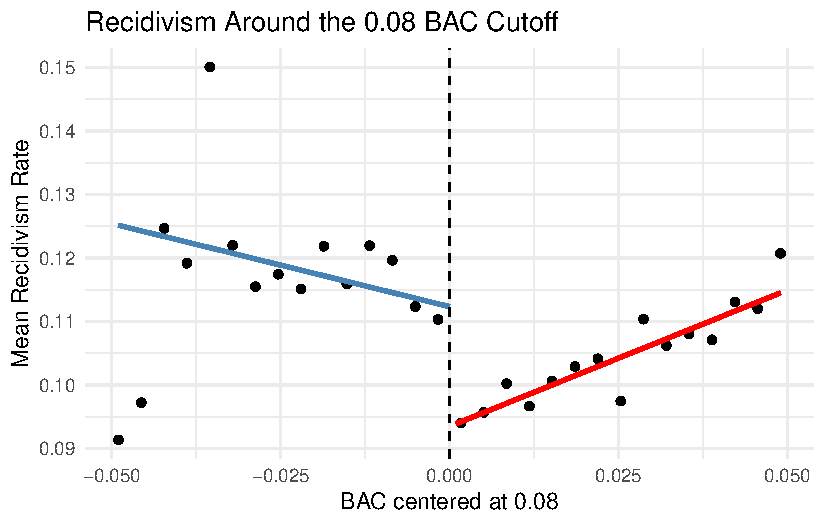
\includegraphics[keepaspectratio]{DTC_Group1-1_files/figure-pdf/unnamed-chunk-11-1.pdf}}

\emph{Figure} \emph{9. RD plot of recidivism around 0.08 cutoff.}

Figure 9 presents a binned scatter plot of recidivism rates against BAC
centered at the 0.08 legal threshold. Each point represents the mean
recidivism rate within a small BAC bin, while the fitted lines show
local linear trends on either side of the cutoff. The vertical dashed
line marks the legal threshold. The figure shows a visible downward jump
in recidivism immediately after the cutoff, indicating that drivers just
above 0.08 have lower subsequent recidivism than those just below it.
This visual pattern is consistent with the deterrence effect estimated
in the regression results.

\begin{enumerate}
\def\labelenumi{\arabic{enumi}.}
\setcounter{enumi}{7}
\tightlist
\item
  \textbf{ii. Results and Interpretation}
\end{enumerate}

Putting the results together, the evidence consistently points to a
deterrent effect at the 0.08 BAC cutoff. Across the main specification,
the narrower bandwidth check, and the model with demographic controls,
the estimated coefficient on above\_08 remains negative and
statistically significant. The preferred interpretation is that drivers
just above 0.08 have a recidivism rate roughly 1.3 to 1.9 percentage
points lower~than comparable drivers just below the cutoff. Because this
pattern is stable across reasonable specifications, the findings support
the conclusion that the harsher DUI punishment triggered at 0.08 reduces
future drunk-driving recidivism for drivers near the legal threshold.

\subsection{9. Limitations}\label{limitations}

While the regression discontinuity design provides credible causal
identification near the cutoff, the estimates should be interpreted as
local effects. Specifically, the results describe the behavior of
drivers whose BAC levels fall very close to the 0.08 threshold and may
not generalize to drivers with substantially higher or lower BAC levels.
In addition, the policy change captured by the cutoff represents a
bundle of sanctions, including fines, license suspension, and potential
jail time, making it difficult to isolate which component drives the
deterrence effect. Despite these limitations, the smooth density of the
running variable and the placebo test results support the credibility of
the RD design.

\subsection{10. Conclusion}\label{conclusion}

These findings suggest that legal thresholds in DUI policy can play an
important deterrent role. Even relatively small increases in punishment
at the legal limit appear to reduce the likelihood of repeat offenses
among drivers near the threshold.

\begin{verbatim}
\end{verbatim}




\end{document}
